\begin{graphicspathcontext}{{./chapters/simulation/imgs/},{./chapters/simulation/imgs/auto/},\old}

\sidecite{Ricci2005}
\begin{frame}{Why a New Abstraction for Multiagent Systems?}
	\begin{columns}
		\begin{column}{.6\linewidth}
			\begin{block}{Classical view of Multiagent Systems}
				\begin{compactitemize}
				\item Agents communicate \emph{directly} via messages
				\item \emph{Environment} is often reduced to a passive data store
				\item Coordination is hard-coded inside each agent
				\item Scalability and reusability suffer
				\end{compactitemize}
			\end{block}
			\begin{block}{Observed problems}
				\begin{compactitemize}
				\item Tight coupling between agents
				\item Difficult to reuse coordination logic across systems
				\item No clear separation between \emph{computation} and \emph{coordination}
				\end{compactitemize}
			\end{block}
		\end{column}
		\begin{column}{.4\linewidth}
			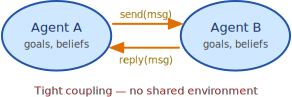
\includegraphics{artifact_classical_mas}
		\end{column}
	\end{columns}
\end{frame}

\sidecite{Ricci2005}
\begin{frame}[t]{Inspiration: Human Work Environments}
	\begin{columns}
		\begin{column}{.6\linewidth}
			\begin{block}{Key observation \cite{Norman1991, Amant2005}}
				In human organisations, people do not only \emph{talk} to each other. \\
				They \Emph{use tools, share resources, read/write shared documents}
			\end{block}
			\begin{compactitemize}
			\item A \emph{pencil}, a \emph{whiteboard}, a \emph{phone} --- these are \emph{mediators} of coordination
			\item Tools provide \Emph{affordances}: defined ways of being used
			\item Tools carry \Emph{observable state} available to all users
			\item Tools can \Emph{react} to use (a phone rings after a call)
			\end{compactitemize}
			\(\Rightarrow\) Can we bring the same idea into MAS?
		\end{column}
		\begin{column}{.4\linewidth}
			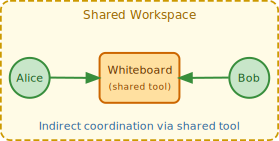
\includegraphics{artifact_human_workspace}
		\end{column}
	\end{columns}
\end{frame}

\sidecite{Omicini2008}
\begin{frame}{{A\&A Paradigm:} Origins}
	\cite{Omicini2008}
	\begin{enumerate}
	\item Proposed as a \Emph{meta-model} for MAS engineering
	\item Provides a \Emph{first-class role} to the environment
	\item Separates \emph{agent logic} (autonomy, deliberation) from \emph{environment services} (coordination, tools)
	\item Inspired by \Emph{Activity Theory} and \Emph{Situated Cognition}
	\item Formalised and implemented in the \Emph{CArtAgO} infrastructure
	\end{enumerate}
\end{frame}

\sidecite{Omicini2008}
\begin{frame}{{Two} First-Class Abstractions}
	\begin{columns}[T]
		\begin{column}{.5\linewidth}
			\begin{block}{Agent}
			\begin{itemize}
			\item \Emph{Autonomous} entity
			\item Has its own \emph{goals} and \emph{reasoning cycle}
			\item Perceives the environment through its \Emph{senses}
			\item Acts on the environment through \Emph{operations} on artifacts
			\item Communicates by \emph{using} shared artifacts
			\end{itemize}
			\end{block}
		\end{column}
		\begin{column}{.5\linewidth}
			\begin{block}{Artifact}
			\begin{itemize}
			\item \Emph{Non-autonomous} resource or tool
			\item Provides a set of \Emph{operations} (usage interface)
			\item Exposes \Emph{observable properties} (observable state)
			\item May generate \Emph{signals} (events)
			\item Resides in a \Emph{workspace}
			\end{itemize}
			\end{block}
		\end{column}
	\end{columns}
	\vspace{.25cm}
	\begin{center}
	\Large $\text{MAS} = \text{Agents} + \text{Artifacts} + \text{Workspaces}$
	\end{center}
\end{frame}

\begin{frame}{Artifacts in Detail}
	\begin{columns}
		\begin{column}{.7\linewidth}
			An artifact is defined by:
			\begin{description}
			\item[Operations] Actions that agents can invoke on the artifact. \\
				Ex: \code{inc()}, \code{reset()}, \code{push(item)}
			\item[Observable Properties] Named observable state variables. \\
				Ex: \code{count(5)}, \code{status("idle")}
			\item[Signals / Events] Proactive notifications emitted by the artifact. \\
				Ex: \code{overflow}, \code{newItem(x)}
			\item[Link Interface] For composition: artifacts can invoke operations on linked artifacts.
			\end{description}
		\end{column}
		\begin{column}{.3\linewidth}
			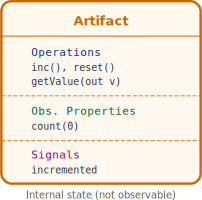
\includegraphics{artifact_structure}
		\end{column}
	\end{columns}
\end{frame}

\sidecite{Omicini2008}
\begin{frame}{{Agents and Artifacts:} Interactions}
	\begin{columns}
		\begin{column}{.6\linewidth}
			\begin{block}{Agent \(\rightarrow\) Artifact (action)}
				\begin{compactitemize}
				\item Agent \Emph{executes an operation} on an artifact
				\item Artifact \Emph{processes} the operation (possibly guarded)
				\item Artifact \Emph{updates} its observable properties
				\item Artifact may \Emph{emit a signal}
				\end{compactitemize}
			\end{block}
			\begin{block}{Artifact \(\rightarrow\) Agent (perception)}
				\begin{compactitemize}
				\item Agent can \Emph{focus} on an artifact
				\item Changes to observable properties generate \Emph{percepts}
				\item Signals are received as \Emph{percepts/events}
				\end{compactitemize}
			\end{block}
		\end{column}
		\begin{column}{.4\linewidth}
			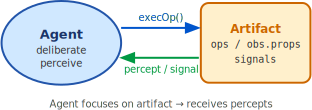
\includegraphics{agent_artifact_interaction}
		\end{column}
	\end{columns}
\end{frame}

\sidecite{Omicini2008}
\begin{frame}{Workspaces}
	\begin{columns}
		\begin{column}{.6\linewidth}
			\begin{definitionblock}{Workspace \cite{Omicini2008}}
				\emph{Container} for artifacts and agents. It defines the \Emph{scope} of interactions and perceptions
			\end{definitionblock}
			\begin{block}{Properties of workspaces}
				\begin{compactitemize}
				\item An agent can \textbf{join} one or more workspaces.
				\item Artifacts are \textbf{created}, \textbf{looked up}, and
				\textbf{disposed} within workspaces.
				\item Workspaces can be \textbf{distributed} across nodes.
				\item Default workspace: \texttt{default}.
				\end{compactitemize}
			\end{block}
			\begin{block}{Key operations for agents}
				\code{makeArtifact}, \code{lookupArtifact}, \code{focus},
				\code{joinWorkspace}
			\end{block}
		\end{column}
		\begin{column}{.4\linewidth}
			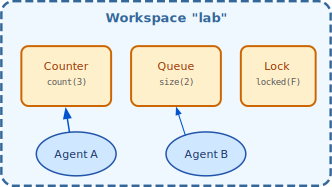
\includegraphics{artifact_workspace}
		\end{column}
	\end{columns}
\end{frame}

\begin{frame}{{Formal Definition} of an Artifact}
	\begin{definitionblock}{Artifact}
		\[
		\mathcal{A} = \langle \mathit{id},\; \mathit{OpSet},\;
		\mathit{ObsPropSet},\; \mathit{SignalSet},\;
		\mathit{State},\; \mathit{LinkSet} \rangle
		\]
	\end{definitionblock}
	\begin{description}
	\item[$\mathit{id}$] Unique identifier (name + workspace)
	\item[$\mathit{OpSet}$] Set of \emph{operations} $\{op_1, op_2, \ldots\}$ each described by a signature and a body (guard + effect)
	\item[$\mathit{ObsPropSet}$] Set of observable properties $\{p_i(\vec{v}_i)\}$ (named, typed, valuated)
	\item[$\mathit{SignalSet}$] Set of signal descriptors the artifact can emit
	\item[$\mathit{State}$] Internal (non-observable) state
	\item[$\mathit{LinkSet}$] Linked artifacts for operation delegation
	\end{description}
\end{frame}

\begin{frame}{{Formal Definition:} Operations and Guards}
	\begin{definitionblock}{Operation}
		\[
		op(\vec{p}) = \langle \mathit{Guard}(\vec{p}, S),\;
		\mathit{Effect}(\vec{p}, S) \rangle
		\]
	\end{definitionblock}
	\begin{description}
	\item[Guard] a predicate on parameters and state. \\
		The operation is \emph{blocked} until the guard is satisfied
	\item[Effect] a function that updates the state and observable properties, and may emit signals
	\end{description}
	\begin{exampleblock}{Counter artifact}
		\begin{itemize}
		\item $\mathit{ObsPropSet} = \{\texttt{count}(n)\}$, initially $n = 0$
		\item $\texttt{inc}() \;=\; \langle \top,\; \texttt{count}(n) \leftarrow \texttt{count}(n{+}1) \rangle$
		\item $\texttt{reset}() \;=\; \langle \top,\; \texttt{count}(n) \leftarrow \texttt{count}(0) \rangle$
		\end{itemize}
	\end{exampleblock}
\end{frame}

\begin{frame}{{Agent Perception \& Action Cycle} in A\&A}
	\begin{columns}
		\begin{column}{.6\linewidth}
			\begin{block}{Agent reasoning cycle}
				\begin{enumerate}
				\item[Perceive] read observable properties of focused artifacts; receive signals as percepts
				\item[Deliberate] update beliefs, select intention
				\item[Act] invoke an operation on an artifact or communicate
				\item[Wait] operation executes asynchronously; agent may receive \emph{feedback}
				\end{enumerate}
			\end{block}
			\begin{block}{Key difference from classical MAS}
				Actions are \emph{delegated to artifacts}; agents do not directly modify the environment
			\end{block}
		\end{column}
		\begin{column}{.4\linewidth}
			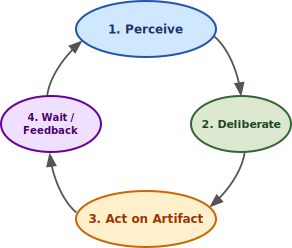
\includegraphics{artifact_agent_cycle}
		\end{column}
	\end{columns}
\end{frame}

\end{graphicspathcontext}
